%======================================================================
\section{Linealización, sistemas lineales e incertidumbre}\label{sec:fundamentos}
%======================================================================

\subsection{Linealizar: la expansión de Taylor de la dinámica}
Cerca de un punto de operación $(\bar x,\bar d,\bar u)$, la dinámica no lineal se reemplaza por
su aproximación de primer orden:
\[
f(x,d,u)\approx\bar f+A(x-\bar x)+B(u-\bar u)+E(d-\bar d),\qquad
A=\tfrac{\partial f}{\partial x},\ B=\tfrac{\partial f}{\partial u},\ E=\tfrac{\partial f}{\partial d}.
\]
Las matrices $A$ (17$\times$17), $B$ y $E$ (17$\times$1) son jacobianos, y aquí se calculan con
diferenciación automática a partir de la misma función del ROM. En el ROM, $B=e_{\Delta M}$: el
caudal del ACS sólo aparece en la ecuación del inventario. El error de la aproximación es de
segundo orden en la distancia al punto: es pequeño mientras la trayectoria no se aleje mucho.
Conviene escribir el modelo lineal en \emph{desviaciones}, $\delta=x-\bar x$, para no restar
números enormes, del orden de $10^{16}$.

\subsection{Sistemas lineales y función de transferencia}
Si $A$, $B$ y la salida $\hat y=C\delta+D\,\Delta u$ son constantes, el sistema es lineal e
invariante en el tiempo (LTI). Su respuesta a una entrada sinusoidal de frecuencia $\omega$
se describe con la \textbf{función de transferencia}
\[
G(s)=C(sI-A)^{-1}B+D,\qquad s=i\omega,
\]
que da la ganancia $|G(i\omega)|$ y el desfase $\arg G(i\omega)$ entre la entrada y la salida.
Es la herramienta clásica del análisis de reactores; por ejemplo, Zhang et al.\ construyen
funciones de transferencia de un reactor de agua a presión linealizando sus ecuaciones de
conservación~\cite{zhang2022}. Para el SMDFR, la figura~\ref{fig:bode} muestra $G$ desde el caudal
del ACS hasta la PCT.

\begin{figure}[H]\centering
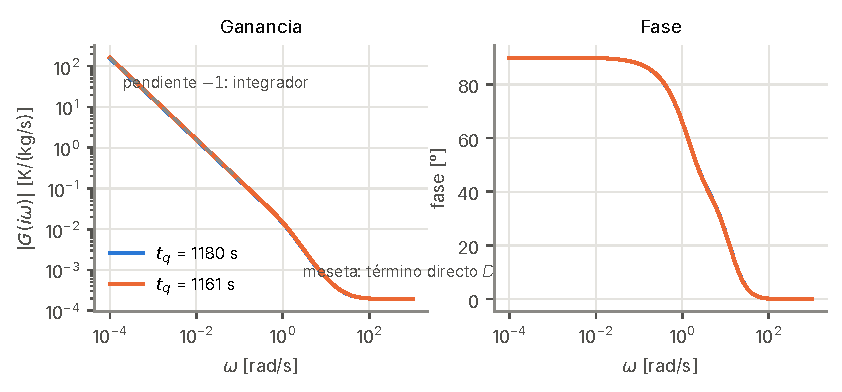
\includegraphics[width=\linewidth]{figures/did_bode.pdf}
\caption{Respuesta en frecuencia del ROM linealizado, desde el caudal del ACS hasta la PCT. A
bajas frecuencias la ganancia cae con pendiente $-1$ y la fase es de $+90°$: es la firma de un
integrador. A altas frecuencias queda una meseta pequeña, el efecto directo del caudal sobre
la corrección $p_4$. Las dos consultas son casi idénticas.}
\label{fig:bode}
\end{figure}

\noindent La lectura física es directa. El caudal del ACS no enfría por sí mismo: suma
inventario, y el inventario es la integral del caudal. Con $\partial\hat y/\partial\Delta
M\approx-1.6\cdot10^{-2}$~K/kg, resulta $G(s)\approx G_M/s$: inyectar 1~kg/s adicional durante
$t$ segundos baja la PCT unos $0.016\,t$~K. Es una regla útil para verificar órdenes de magnitud.
La diferencia entre el caudal máximo y el mínimo del ACS es de 12.3~kg/s, que durante los 12.5~s
del horizonte suman unos 150~kg y bajan la PCT unos 2.4~K. Es lo mismo que mide el modelo no
lineal en la figura~\ref{fig:autoridad}. Y de aquí sale la estrategia óptima: \emph{acumular
inventario lo antes posible}, porque el caudal inyectado al principio del horizonte sigue
actuando durante todo el resto.

\subsection{Programación cuadrática y dualidad}
Con el modelo lineal, el costo cuadrático y las restricciones lineales, P0 se convierte en un
\textbf{programa cuadrático} (QP). Si su hessiana es semidefinida positiva, el QP es convexo y,
por la proposición~\ref{prop:convexo}, todo mínimo local es global. Los QP convexos se resuelven
con métodos de punto interior especializados, como Clarabel~\cite{goulart2024}, que además
entregan un certificado.

\begin{proposicion}[Dualidad débil y certificado del QP]\label{prop:dual}
Para un QP convexo $p^\star=\min\{\tfrac12z^\top Pz+q^\top z:\ Az\le b,\ Fz=g\}$ y su función
dual $g(\lambda,\nu)=\inf_zL(z,\lambda,\nu)$, con
$L=\tfrac12z^\top Pz+q^\top z+\lambda^\top(Az-b)+\nu^\top(Fz-g)$, se cumple $g(\lambda,\nu)\le p^\star$
para todo $\lambda\ge0$. Por lo tanto, si un par primal-dual factible tiene brecha
$p(z)-g(\lambda,\nu)\le\eta$, la solución $z$ es óptima con error a lo más $\eta$.
\end{proposicion}
\begin{proof}
Para todo $z$ factible y $\lambda\ge0$ se tiene $L(z,\lambda,\nu)\le p(z)$, porque
$\lambda^\top(Az-b)\le0$ y $Fz-g=0$. Minimizando en $z$, $g(\lambda,\nu)\le L(z,\lambda,\nu)\le
p(z)$, y tomando el ínfimo sobre $z$ factible, $g\le p^\star\le p(z)$~\cite{boyd2004}.
\end{proof}
\noindent Este certificado vale para el \emph{modelo lineal}: dice que el QP quedó bien
resuelto, no que su decisión sea buena para el problema no lineal. Esa pregunta se responde en
la sección~\ref{sec:certteoria}.

\subsection{Incertidumbre: de dónde viene y cómo se representa}
El controlador decide sin conocer el futuro. Hay dos tipos de incertidumbre:
\begin{itemize}
  \item \textbf{continua}: la fuga futura, que se pronostica con error, y el error del propio
        ROM frente a la planta;
  \item \textbf{discreta}: si el ACS fallará o no, y cuándo.
\end{itemize}
Las herramientas para incorporarla en la decisión, de menor a mayor costo, son tres.

\paragraph{Restricción probabilística.} En lugar de exigir $\hat y_k\le U_y$, que no tiene
sentido si $\hat y_k$ es aleatoria, se exige que la probabilidad de violarla sea pequeña,
$\mathbb P(\hat y_k>U_y)\le\varepsilon$~\cite{charnes1959}.

\begin{proposicion}[Restricción probabilística gaussiana]\label{prop:cc}
Si $\hat y_k=\bar y_k(u)+c_k^\top w$ con $w\sim\mathcal N(0,\Sigma)$, entonces
$\mathbb P(\hat y_k>U_y)\le\varepsilon$ si y sólo si $\bar y_k(u)+z_{1-\varepsilon}\sigma_k\le U_y$,
con $\sigma_k^2=c_k^\top\Sigma c_k$ y $z_{1-\varepsilon}$ el cuantil de la normal estándar.
\end{proposicion}
\begin{proof}
$\hat y_k\sim\mathcal N(\bar y_k,\sigma_k^2)$, así que
$\mathbb P(\hat y_k>U_y)=1-\Phi\big((U_y-\bar y_k)/\sigma_k\big)\le\varepsilon$ equivale a
$(U_y-\bar y_k)/\sigma_k\ge z_{1-\varepsilon}$.
\end{proof}
\noindent Con el modelo lineal, la fuga entra de forma aditiva y $\sigma_k$ no depende de $u$:
la restricción probabilística es una restricción lineal más ajustada, y el QP sigue siendo un
QP. Con $\varepsilon=0.05$, por ejemplo, se exige $\bar y_k+1.645\sigma_k\le U_y$.

\paragraph{Aproximación por promedio muestral (SAA).} Si la distribución no es gaussiana o el
modelo no es lineal, se reemplaza la esperanza por el promedio sobre $M$ escenarios
muestreados $\hat d^{(1)},\dots,\hat d^{(M)}$~\cite{shapiro2009}:
\[
\min_u\ \mathbb E\big[J(u;\hat d)\big]\approx\min_u\ \frac1M\sum_{j=1}^{M}J(u;\hat d^{(j)}).
\]
Al crecer $M$, el valor y las soluciones convergen a los del problema verdadero. Con $M$ finito,
el óptimo dentro de la muestra es optimista: está sesgado hacia abajo. Por eso las decisiones
se evalúan \emph{fuera de muestra}, con escenarios que no se usaron para optimizar.

\paragraph{Dos etapas y no anticipación.} En el MPC sólo se aplica la primera acción, y las
siguientes se re-optimizarán con información nueva. La versión de \emph{dos etapas} del SAA
refleja eso: la primera acción $u_1$ es común a todos los escenarios, porque se decide antes de
saber cuál ocurrirá (\emph{no anticipación}), y las siguientes pueden adaptarse a cada escenario
(\emph{recurso}).

\paragraph{El escenario óptimo.} Homem-de-Mello et al.\ demostraron que, en una clase de
programas estocásticos de dos etapas con recurso fijo y segunda etapa lineal, existe un
\emph{único escenario} cuyo problema determinista reproduce la decisión
estocástica~\cite{homem2026}. Ese escenario no tiene por qué ser único ni pertenecer al soporte
de la distribución. El ejemplo clásico es el del vendedor de diarios (\emph{newsvendor}), que
debe decidir cuántos diarios comprar sin conocer la demanda. La compra óptima es un
\emph{cuantil} de la demanda, así que basta resolver el problema determinista con ese cuantil
como demanda. Si un resultado así valiera para el MPC, el riesgo de pronóstico podría tratarse
resolviendo el problema con un pronóstico bien elegido, sin multiplicar los escenarios. Para
eso el problema debe ser lineal, y ésa es otra razón para disponer de una versión lineal de
P0.

\takeaway{\textbf{Para recordar.} Linealizar convierte P0 en un QP convexo, con óptimo global,
certificado dual y una función de transferencia que explica la física: el ACS actúa a través de
un integrador. La incertidumbre se incorpora con restricciones probabilísticas, que siguen
siendo lineales si el modelo es lineal, o con escenarios (SAA), en cuyo caso el tamaño del
problema crece con su número.}
